\chapter{Introducción}


\section{Fundamentos teóricos de la luz}

\subsection{Radiación electromagnética}

La luz es radiación electromagnética que se propaga en forma de onda a través del espacio transportando energía radiante en el proceso. Está constituida por partículas elementales sin masa denominadas fotones.
Las propiedades de la luz están condensadas en el espectro electromagnético (Figura~\ref{espectroelectromagnetico}) con base en el número de oscilaciones de la onda por unidad de tiempo (frecuencia, $\nu$) y la distancia lineal entre dos puntos equivalentes de ondas sucesivas (longitud de onda, $\lambda$).\\

\begin{figure}
  \centering
    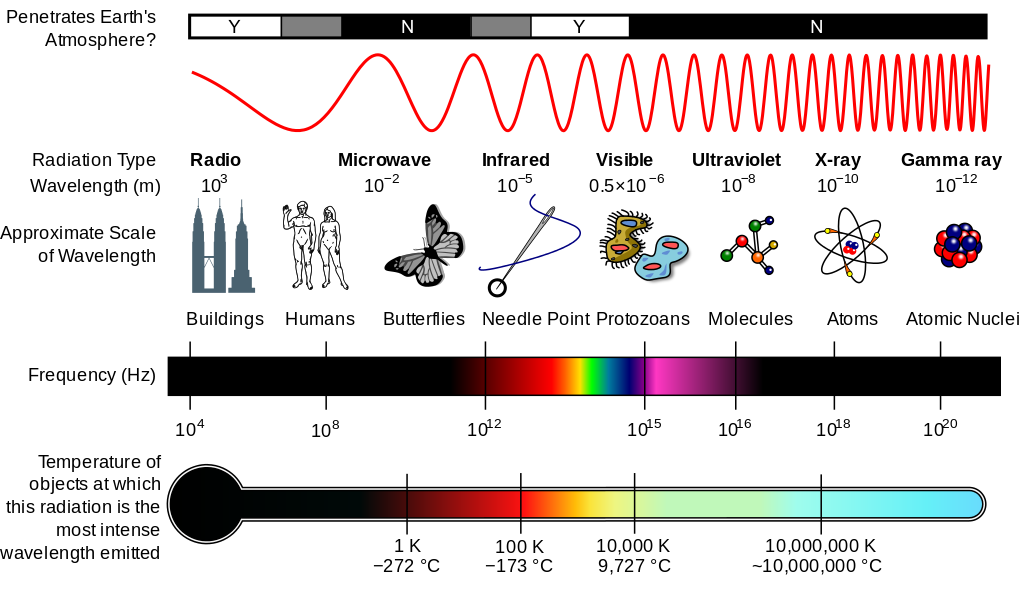
\includegraphics[width=1\textwidth]{espectroelectromagnetico}
  \caption{Espectro electromagnético \citep{NASA2007}}
  \label{espectroelectromagnetico}
\end{figure}

Una de tales propiedades de interés para este trabajo en la región visible del espectro electromagnético ($\sim$ 450-750 nm), es la temperatura de color ($T$)  que está definida a partir de la Ley de desplazamiento de Wien. Esta ley explica la relación inversa entre la longitud de onda en la que se produce el pico de emisión de un cuerpo negro ($\lambda_{max}$) y $T$:

\begin{equation}
\lambda_{max}=\dfrac{b}{T}
\end{equation}

Donde $b = 2.897...\e{-3}$ m K, es denominada la constante de Wien. Un cuerpo negro es un objeto ideal que absorbe toda radiación electromagnética incidente y que en equilibrio termodinámico y térmico, emite radiación térmica sólo con dependencia en su temperatura.\\

En la \textbf{Sección \ref{fuentesluz}} se presenta la aplicación del concepto de temperatura de color para la clasificación del color de las fuentes de luz y su implicación biológica en los seres vivos.\\

\subsection{Propiedades ópticas}

La óptica es el campo de la física que se encarga de estudiar la interacción de la luz con la materia. En la  \textbf{Tabla \ref{tab:propiedadesopticas}} se resumen las principales propiedades ópticas.\\


\begin{table}[]
\centering
\caption{Propiedades ópticas de la luz}
\label{tab:propiedadesopticas}
\resizebox{\textwidth}{!}{%
\begin{tabular}{lll}
\hline
\textbf{Propiedad} &          & \textbf{Descripción}                                             \\ \hline
                                    &          &                                                                                   \\
Absorción                           &          & La luz es captada en el objeto y aumenta su energía térmica                       \\
                                    &          &                                                                                   \\
Transmisión                         &          & La luz atraviesa el objeto sin cambio de dirección ni intensidad                  \\
                                    &          &                                                                                   \\
Dispersión                          &          & La luz es captada en el objeto y se re-emite con diferente dirección e intensidad \\
                                    &          &                                                                                   \\
                                    & Rayleigh & Dispersión elástica (conserva energía) en que la longitud de onda de la luz       \\
                                    &          & incidente es mucho mayor que el tamaño del objeto                                 \\
                                    &          &                                                                                   \\
                                    & Mie      & Dispersión elástica en que la longitud de onda de la luz incidente es similar     \\
                                    &          & al tamaño del objeto                                                              \\
                                    &          &                                                                                   \\
Reflexión                           &          & La luz se desvía al chocar con el objeto con un ángulo igual al de incidencia     \\
                                    &          &                                                                                   \\
Refracción                          &          & La luz cambia de dirección y velocidad al atravesar por un medio diferente       
\end{tabular}%
}
\end{table}

\subsection{Unidades de medición}

Existen dos campos de estudio que se encargan de la medición de la luz: la fotometría y la radiometría. La fotometría se encarga de medir la luz con base en la sensibilidad de la vista humana. Por otro lado, la radiometría mide la luz abarcando todas las longitudes de onda del espectro electromagnético. Al ser de carácter general este trabajo, en la \textbf{Tabla \ref{tab:unidadesradiometria}} se muestran las unidades del Sistema Internacional de Unidades (SI) utilizadas en radiometría. 

\begin{table}[]
\centering
\caption{Unidades del SI utilizadas en radiometría}
\label{tab:unidadesradiometria}
\resizebox{\textwidth}{!}{%
\begin{tabular}{lll}
\hline
\textbf{Magnitud física}            & \textbf{Unidad del SI}                      & \textbf{Notas}                                                    \\ \hline
                                    &                                             &                                                                   \\
Energía radiante (Q)                & julio (J)                                   & Energía                                                           \\
                                    &                                             &                                                                   \\
Flujo radiante ($\Phi$)             & vatio                                       & Energía radiada por unidad de tiempo (potencia)                   \\
                                    &                                             &                                                                   \\
Intensidad radiante (I)             & vatio por estereorradián                    & Potencia por ángulo sólido                                        \\
                                    &                                             &                                                                   \\
Irradiancia (E)                     & vatio por metro cuadrado                    & Potencia incidente por superficie                                 \\
                                    &                                             &                                                                   \\
Emitancia radiante (M)              & vatio por metro cuadrado                    & Potencia emitida por superficie de la fuente radiante             \\
                                    &                                             &                                                                   \\
Radiancia (L)                       & vatio por estereorradián por metro cuadrado & Potencia por ángulo sólido y por superficie                       \\
                                    &                                             &                                                                   \\
Radiancia espectral ($L_{\lambda}$) & vatio por estereorradián por metro cúbico   & Potencia por ángulo sólido, por superficie y por longitud de onda
\end{tabular}%
}
\end{table}

Métodos experimentales y métodos teóricos


\section{Brillo del cielo nocturno}

\subsection{Componentes del brillo del cielo nocturno}

De acuerdo con Leinert at.al (1998), el brillo total $(I_{tot})$ del cielo nocturno puede calcularse a partir de la siguiente ecuación:

\begin{equation}\label{eq:ej}
I_{tot}=(I_A + I_{ZL} + I_{ISL} + I_{DGL} + I_{EBL})\ exp \ (-\tau) + I_{SCA}
\end{equation}

Donde $\tau$ es el coeficiente de extinción que depende de la longitud de onda, el ángulo cenital, la altura sobre el nivel del mar y la composición atmosférica del lugar de la observación.


\subsection{Variación natural del brillo del cielo nocturno por influencia de objetos astronómicos}

\subsection{Variación natural del brillo del cielo nocturno por influencia de las condiciones atmosféricas}

\subsubsection{Propiedades ópticas de las nubes}

\subsubsection{Propiedades ópticas del aerosol atmosférico}


\section{Importancia del ciclo día-noche en la evolución de la vida}

La duración del ciclo día-noche en la Tierra ha cambiado significativamente a lo largo de la historia geológica debido a la variación de la rotación del planeta. La velocidad de rotación original de los planetas  es consecuencia de la conservación del momento angular que poseía la nebulosa interestelar que, al colapsar, dio origen al Sistema Solar hace aproximadamente 4600 Ma \citep{Greaves2005}. Sin embargo, si la hipótesis del Impacto de Theia es correcta, es factible que la rotación primordial de la Tierra haya sido reconfigurada hace alrededor de 4500 Ma, cuando un cuerpo astronómico del tamaño de Marte, nombrado Theia, colisionó tangencialmente con nuestro planeta dando origen, además, a la Luna \citep{Stevenson1987}.\\

La masa lunar es lo suficientemente grande y cercana con respecto a la Tierra para ejercer atracción gravitatoria significativa sobre los océanos, generando así abultamientos de masas de agua (mareas) en ambos extremos del planeta alineados con el eje Tierra-Luna. Sin embargo, la rotación terrestre ocasiona el arrastre de las mareas hacia delante del mencionado eje, lo que implica que una fracción de la atracción gravitatoria Tierra-Luna está desfasada y da origen al torque lunar $\uptau_0$ que reduce la velocidad de rotación de la Tierra \citep{Conway1982}.\\ 

Como se muestra en la Figura~\ref{duraciondia}, la duración que tuvo el día terrestre posterior a la gran colisión de Theia debió de ser de tan sólo 7 horas aproximadamente gracias a la gran velocidad de rotación y el cambio en la inclinación del eje de rotación que el planeta llegó a experimentar luego del evento \citep{Stevenson&Bartlett2016}, \citep{Stevenson1987}; con el paso de los millones de años, tal velocidad fue disminuyendo como consecuencia del torque lunar \citep{Conway1982}.\\ 

El periodo estable de duración del día terrestre de 21 horas que se mantuvo durante gran parte del Precámbrico (Figura~\ref{duraciondia}) se explica con la llamada Hipótesis de Estabilización Resonante \citep{Zahnle&Walker1987}, la cual sostiene que, durante algún tiempo, el anteriormente mencionado torque lunar pudo haber sido cancelado por un torque de signo contrario originado por la resonancia entre las mareas atmosféricas semi-diurnas térmicamente accionadas y las oscilaciones libres de la atmósfera.\\

\begin{figure}
  \centering
    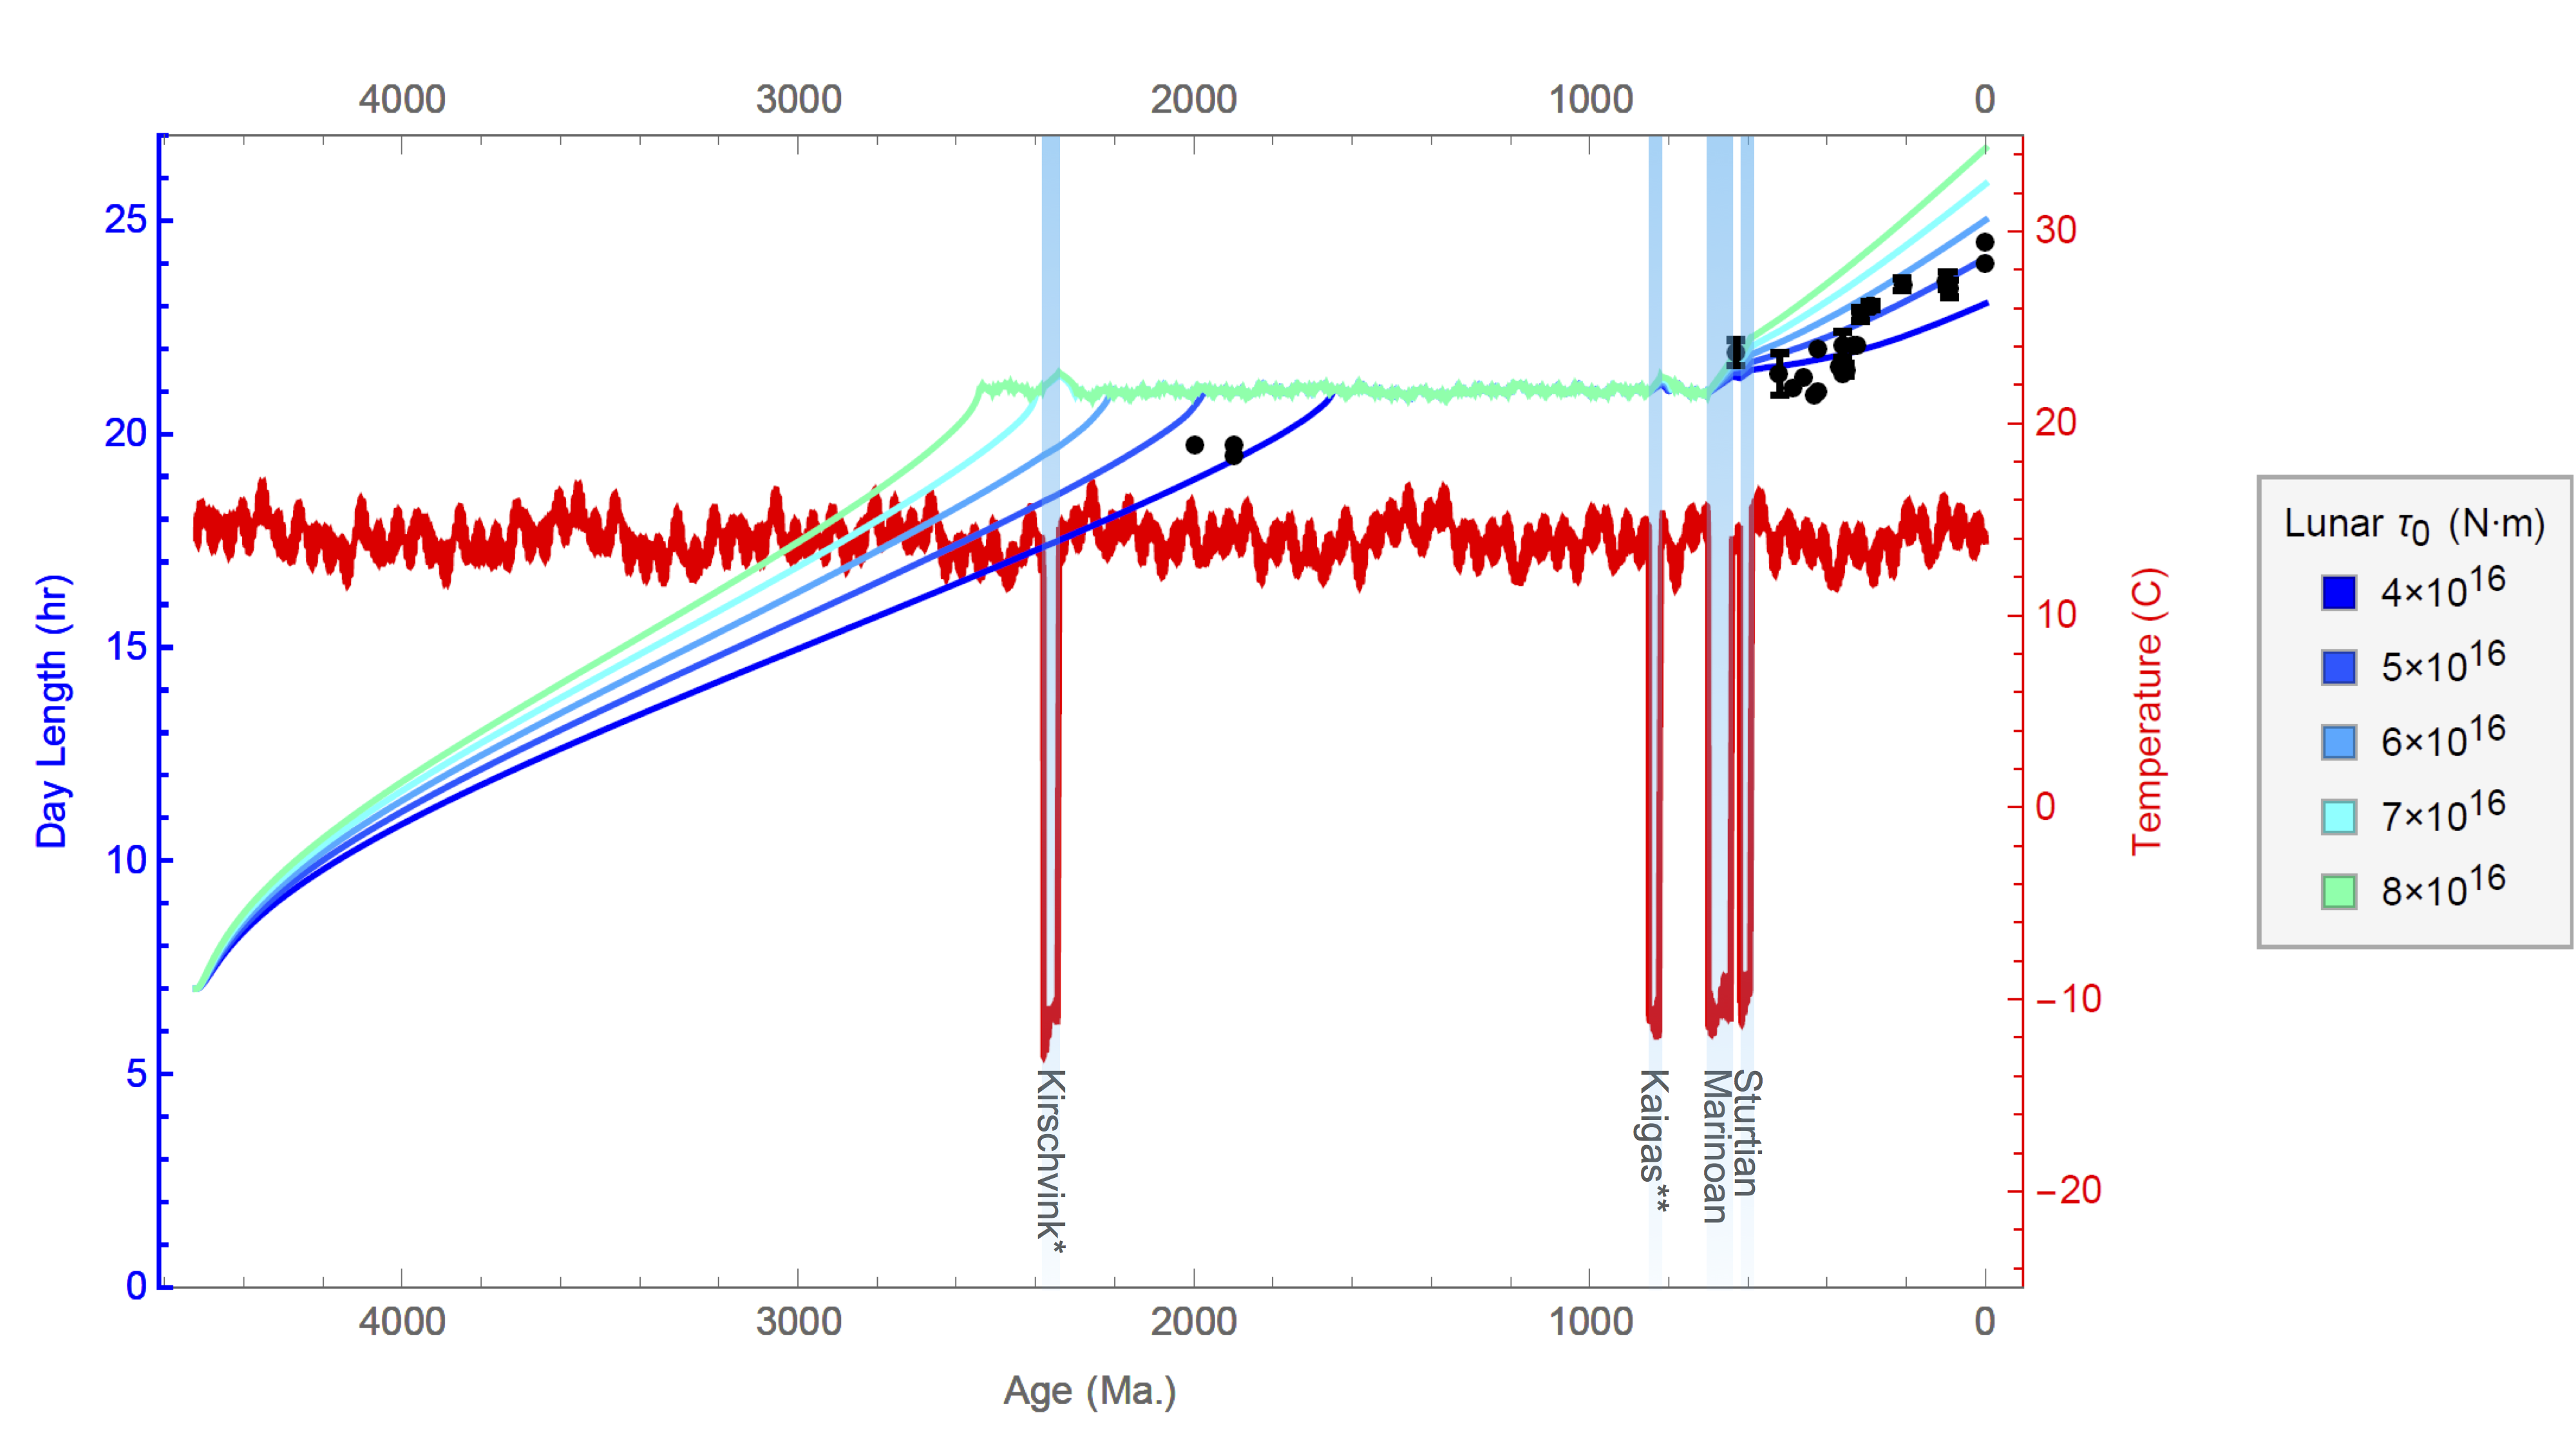
\includegraphics[width=1\textwidth]{duraciondeldiahistorico}
  \caption{Simulación de la historia geológica de la duración del día terrestre \citep{Stevenson&Bartlett2016}}
  \label{duraciondia}
\end{figure}

La velocidad de rotación actual de la Tierra debió comenzarse a perfilar hace aproximadamente 600 Ma cuando las grandes glaciaciones de ese entonces pudieron haber desestabilizado térmicamente el torque atmosférico, por lo que actualmente, el torque lunar sigue siendo lo suficientemente considerable como para continuar disminuyendo la velocidad del planeta \citep{Stevenson&Bartlett2016}. Para el final del Criogénico, el ciclo día-noche tomó, finalmente, su configuración actual al mismo tiempo que los niveles de oxígeno y ozono estratosférico fueron óptimos para el surgimiento y desarrollo de vida más compleja (multicelular) en un evento conocido como \textit{la Radiación del Cámbrico}, durante el que se originaron y diversificaron la mayoría de los filos animales incluyendo el de los cordados, al que pertenecemos los humanos.\\

$https://en.wikipedia.org/wiki/Cambrian_explosion$	
Poner la gráfica de Holker. Oscuridad, ventaja evolutiva. Más horas de noche, mayor nocturnidad con el paso del tiempo.\\

\section{Contaminación lumínica}

\subsection{El enfoque socioecosistémico}

Socioecosistema\\

1. Socioecosistema IES\\

2. De ecosistema a socioecosistema diseñado
como territorio del capital agroindustria\\

3. Sistemas socio-ecológicos: elementos teóricos y conceptuales para la discusión en torno a vulnerabilidad hídrica.\\

Uso y abuso de la energía\\

\subsection{Contexto histórico del estudio de la CL}

\subsection{Tipos de CL}

Skyglow de interés

\subsection{Consecuencias de la CL}

En qué región del espectro se ven afectadas diferentes clases de animales de acuerdo con su visión (luminancia).\\

Podrían estimular la nucleación de partículas ultrafinas que se forman por reacciones fotoquímicas.

\subsection{Marco regulatorio: normas y leyes en México y el mundo}

Ley 31/1998 Protección de la Calidad Astronómica de los Observatorios del Instituto de Astrofísica de Canarias.\\

Ley 6/2001 Ordenación ambiental del alumbrado para la protección del medio nocturno.\\

Zonificación con 4 categorías y una especial.\\

\begin{itemize}

    \item E1. Espacios que por sus características naturales o su valor astronómico especial, sólo se puede admitir un brillo mínimo.
    
    \item E2. Áreas incluidas en ámbitos territoriales que sólo admiten un brillo reducido.
    
    \item E3. Áreas incluidas en ámbitos territoriales que admiten un brillo medio
    
    \item E4. Áreas incluidad en ámbitos territoriales que admiten un brillo alto.
    
    \item Puntoa de referencia. Puntos cercanos a las áreas de valor astronómico o natural especial incluidos en E1, para los que hay que establecer una regulación específica en función de la distancia a la que se encuentren del área en cuestión.
    
    
\end{itemize}

Según el Departamento de Estudios Luminotécnicos de la ETSEIB (UPC) en \textit{Evaluación del Impacto Ambiental Lumínico en Zonas Protegidas del Área Metropolitana de Barcelona}, los aspectos importantes para controlar la Contaminación Lumínica son:

\begin{itemize}
    \item Niveles más estrictos a los permisos de las luminarias (Comité Internationale d'Eclairage)
    
    \item Límites de luminosidad en el espacio-tiempo (periodo de protección especial a partir de las 23 hrs.)
    
     \item Cambiar el uso de luz blanca (especialmente nociva) a una temperatura de color neutra (4200 K), promoviendo las cálidas (inferiores a 3000 K)
     
\end{itemize}

\section{Alumbrado público}

\subsection{Fuentes de luz} \label{fuentesluz}

Curso de iluminación de Manuel García.\\

En la práctica,la temperatura de color sólo tiene significado físico para objetos que son aproximadamente cuerpos negros.\\

Color temperature Wikipedia.\\

Lámparas incandesentes (el bulbo se aproxima a un cuerpo negro irradiador). \\


Lámparas fluorescentes y LEDS no emiten en el espectro de un cuerpo negro, para esto se aplica la correlated color temperature.\\

\subsection{Tipos de luminarias}

Poste,etc.

\subsection{Función de emisividad urbana}

Teoría de Kocifaj y Héctor

\section{Estudio de caso: Ciudad de México}


\subsection{Descripción del área de estudio}

División política, extensión, situación geográfica, 

Incluir REPSA

\subsection{Inventario de alumbrado público}

Incluir número total de luminarias

\subsection{Consumo de energía eléctrica}


Datos de consumo de energía eléctrica por entidad federativa por el Sistema de Información Energética de la Secretaría de Energía.\\

Su relación con las emisiones de gases de efecto invernadero 

\subsection{Climatología de nubes y aerosol atmosférico}

Artículo de Giovanni Caraballi

\section{Hipótesis}

\section{Objetivos}

\subsection{Generales}

\begin{itemize}

    \item Reproducir el modelo \textit{SkyGlow} para el caso de la Ciudad de México
    
    \item Estimar los niveles de contaminación lumínica en la Ciudad de México 
    
    \item Generar un antecedente para la campaña de validación del modelo \textit{SkyGlow} en la Ciudad de México
    
\end{itemize}

\subsection{Particulares}

\begin{itemize}

    \item Caracterizar el alumbrado público de la Ciudad de México 
    
    \item Elaborar un mapa teórico de contaminación lumínica de la Ciudad de México bajo condiciones de cielo despejado
    
    \item Construir mediante simulaciones diferentes escenarios del brillo del cielo nocturno tomando en cuenta diferentes posiciones del observador y condiciones atmosféricas
    
    \item Inferir la influencia del aerosol atmosférico  y la nubosidad en el brillo del cielo nocturno a partir del objetivo anterior
    
    
\end{itemize}